\documentclass[10pt,a4paper]{article}

\usepackage[utf8]{inputenc}
\usepackage[T1]{fontenc}
\usepackage[spanish, es-tabla]{babel}
\usepackage{lmodern}
\usepackage{csquotes}
\usepackage{amsmath, amsfonts, amssymb, amsthm}
\usepackage{graphicx}
\usepackage{subcaption}
\usepackage{float}

\usepackage[
    left=2.54cm,
    right=2.54cm,
    top=2.54cm,
    bottom=2.54cm
]{geometry}

\usepackage{tikz}
\usepackage{soul}
\usepackage{listings}
\usepackage[most]{tcolorbox}
\usepackage{xcolor}
\usepackage{hyperref}

\tcbset{shield externalize}

\usetikzlibrary{arrows.meta, positioning, automata}
\usetikzlibrary{babel}
\usetikzlibrary{external}

\tikzexternalize[prefix=build-tikz/]



\lstset{
    basicstyle=\footnotesize\ttfamily,
    frame=single,
    numbers=left,
    inputencoding=utf8,
    extendedchars=true,
    breaklines=true,
    showstringspaces=false,
    keywordstyle=\color{blue},
    commentstyle=\color{green!50!black},
    stringstyle=\color{red!70!black}
}


\newtcbtheorem[number within=section]{ejercicio}{Ejercicio}{
    enhanced,
    sharp corners,
    boxrule=0pt,
    leftrule=5pt,
    colframe=gray!30!black,
    colback=gray!5!white,
    coltitle=white,
    fonttitle=\bfseries,
    separator sign={.\ },
    before skip=10pt,
    after skip=10pt
}{ej}



\newtcbtheorem[number within=section]{mytheo}{Teorema}{
    enhanced,
    sharp corners,
    boxrule=0pt,
    leftrule=5pt,
    colframe=blue!40!black,
    colback=blue!5!white,
    coltitle=white,
    fonttitle=\bfseries,
    separator sign={.\ },
    before skip=10pt,
    after skip=10pt
}{th}



\newtcolorbox{alerta}[1]{
    enhanced,
    sharp corners,
    boxrule=0pt,
    leftrule=5pt,
    colframe=red!40!black,
    colback=red!5!white,
    coltitle=white,
    fonttitle=\bfseries,
    title=#1,
    before skip=10pt,
    after skip=10pt
}

\newtcolorbox{nota}[1]{
    enhanced,
    sharp corners,
    boxrule=0pt,
    leftrule=5pt,
    colframe=orange!40!black,
    colback=yellow!5!white,
    coltitle=white,
    fonttitle=\bfseries,
    title=#1,
    before skip=10pt,
    after skip=10pt
}


\begin{document}


\begin{titlepage}

    \centering

    {\huge \textbf{Universidad Nacional Autónoma de México}}\\[0.3cm]

    \rule{\linewidth}{2mm}\\[0.3cm]

    {\large \textbf{Facultad de Estudios Superiores Acatlán}}\\[1cm]

    
\includegraphics[width=6cm]{../../Archivos/Imagenes_Logos/acatlan.png}\\[1cm]

    {\Large \textbf{Matemáticas Aplicadas y Computación}}\\[1cm]

    {\huge \textbf{Database Administrator}}\\[0.5cm]

    \rule{\linewidth}{1mm}\\[0.3cm]

    \vfill

    {\Large \textit{Carga de Datos}}\\[0.5cm]

    \vfill

    \rule{\linewidth}{0.5mm}\\[0.3cm]

    %{\Large \textit{Ricardo López Ramírez}}\\

    \rule{\linewidth}{0.5mm}\\[0.8cm]

    \small

    Actualización: \today

\end{titlepage}



\pagenumbering{roman}

\tableofcontents

\clearpage

\pagenumbering{arabic}

\setcounter{page}{1}


\section{Ruta en Windows}

\vspace{3mm}

\begin{enumerate}

    \item Modifica tu conexión y cambia el usuario actual por
    \texttt{root}. Todo lo que viene a continuación deberá
    ser ejecutado con dicho usuario.

    \item Ejecuta el siguiente comando en MySQL Workbench y
    copia el directorio que aparece como resultado.

\end{enumerate}

\begin{figure}[H]
    \centering
    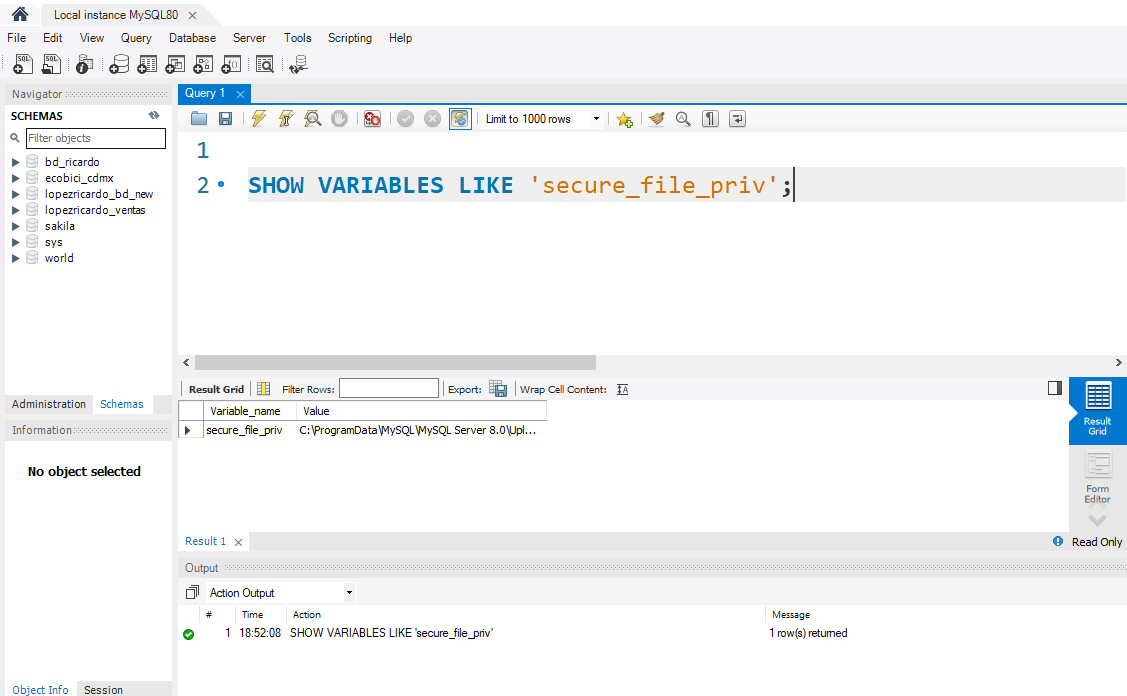
\includegraphics[
        width=0.8\textwidth
    ]{../Actividad_3/Imagen/Show_va.png}
    \caption{Variable \texttt{secure\_file\_priv}}
    \label{fig:secure-file-priv}
\end{figure}

\begin{lstlisting}
'secure_file_priv', 'C:\ProgramData\MySQL\MySQL Server 8.0\Uploads\'
\end{lstlisting}

\vspace{3mm}

\subsection{Mover archivos de texto}

Los archivos TXT se copian en la ruta indicada por la variable
\texttt{secure\_file\_priv}:

\begin{figure}[H]
    \centering
    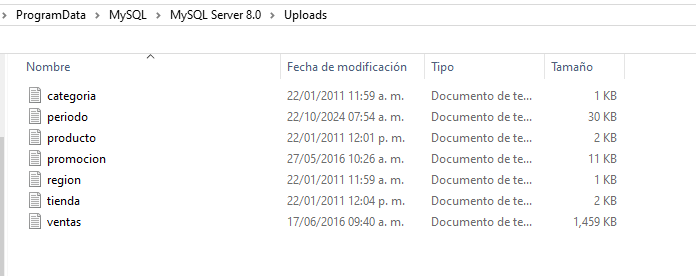
\includegraphics[
        width=0.8\textwidth
    ]{../Actividad_3/Imagen/Mov_ar.png}
    \caption{Movimiento de archivos}
    \label{fig:movimiento-archivos}
\end{figure}

\newpage



\section{Carga de datos directa}

\subsection{Tabla \texttt{categoria}}

\vspace{3mm}

\begin{figure}[H]
    \centering
    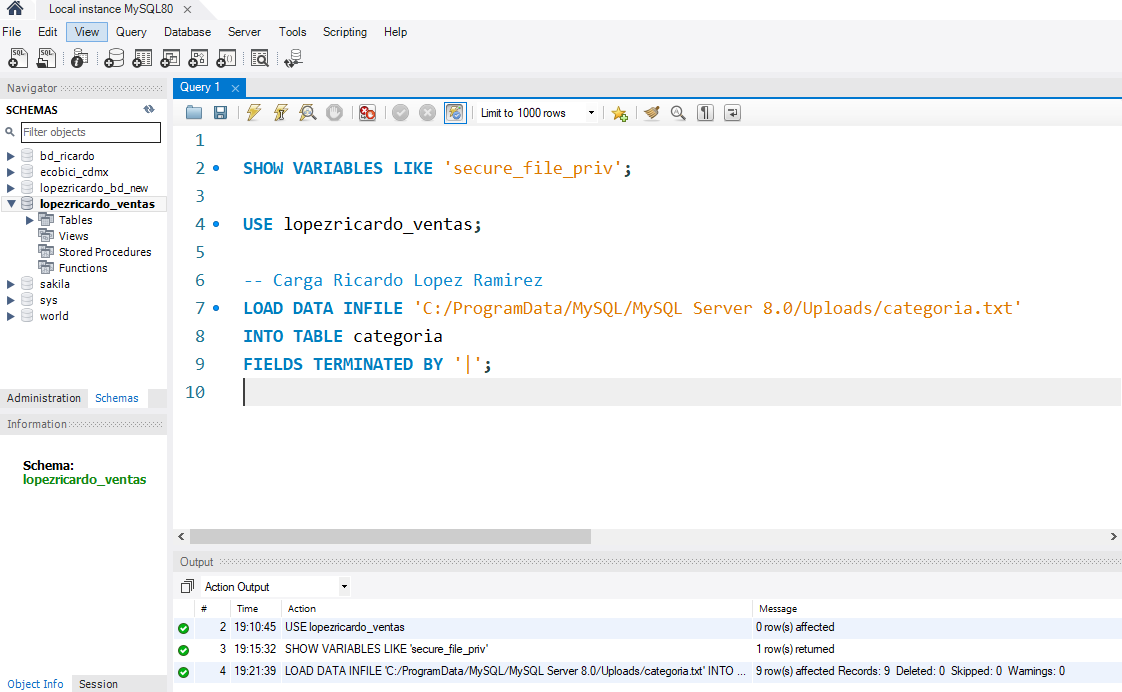
\includegraphics[
        width=0.8\textwidth
    ]{../Actividad_3/Imagen/categoria.png}
    \caption{Tabla categoría}
    \label{fig:tabla-categoria}
\end{figure}



\subsection{Tabla \texttt{producto}}

\vspace{3mm}

\begin{lstlisting}
Error Code: 1406. Data too long for column pkg_tipo at row 22
\end{lstlisting}

\begin{figure}[H]
    \centering
    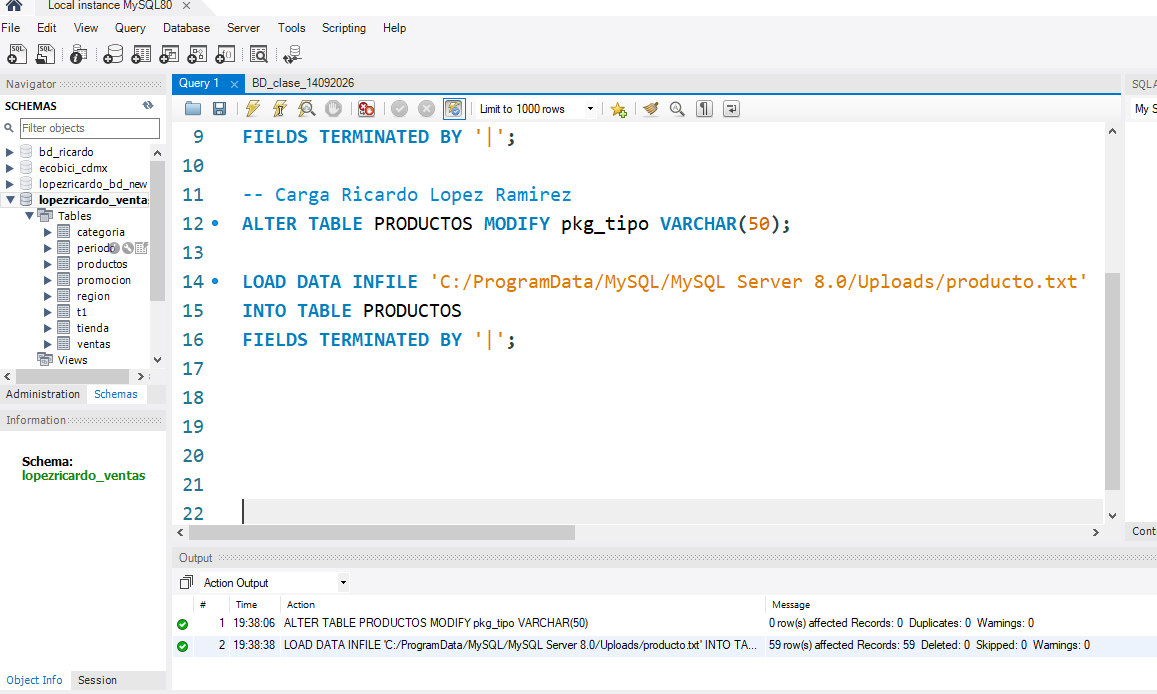
\includegraphics[
        width=0.8\textwidth
    ]{../Actividad_3/Imagen/productos.png}
    \caption{Tabla producto}
    \label{fig:tabla-producto}
\end{figure}


\subsection{Tabla \texttt{region}}

\vspace{3mm}

\begin{figure}[H]
    \centering
    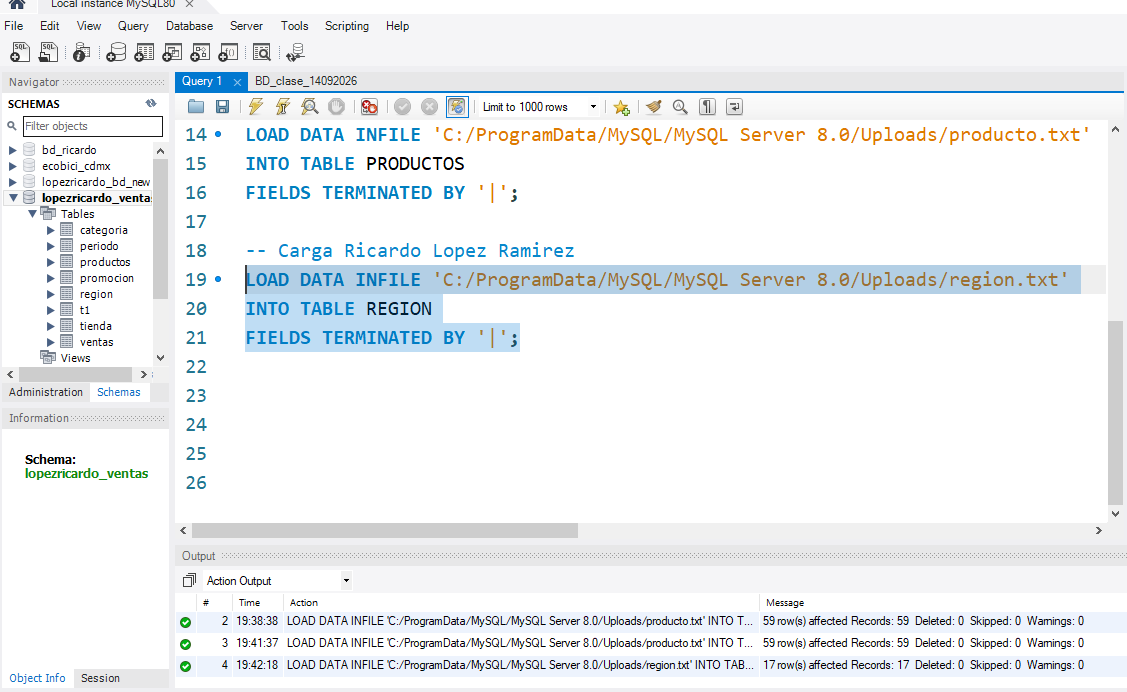
\includegraphics[
        width=0.8\textwidth
    ]{../Actividad_3/Imagen/region.png}
    \caption{Tabla región}
    \label{fig:tabla-region}
\end{figure}


\subsection{Tabla \texttt{tienda}}

\vspace{3mm}

\begin{figure}[H]
    \centering
    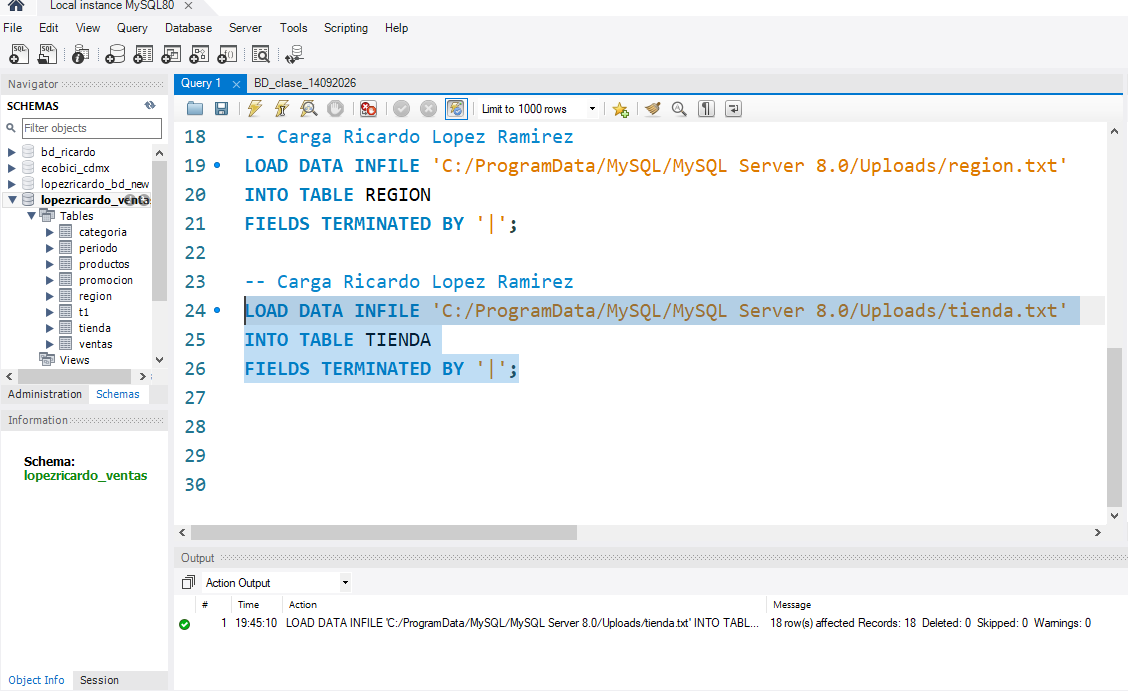
\includegraphics[
        width=0.8\textwidth
    ]{../Actividad_3/Imagen/tienda.png}
    \caption{Tabla tienda}
    \label{fig:tabla-tienda}
\end{figure}

\newpage

\subsection{Tabla \texttt{ventas}}

\vspace{3mm}

\begin{lstlisting}
19:51:22    LOAD DATA INFILE 'C:/ProgramData/MySQL/MySQL Server 8.0/Uploads/ventas.txt' INTO TABLE VENTAS FIELDS TERMINATED BY '|' 69852 row(s) affected Records: 69852 Deleted: 0 Skipped: 0 Warnings: 0 1.078 sec
\end{lstlisting}

\begin{figure}[H]
    \centering
    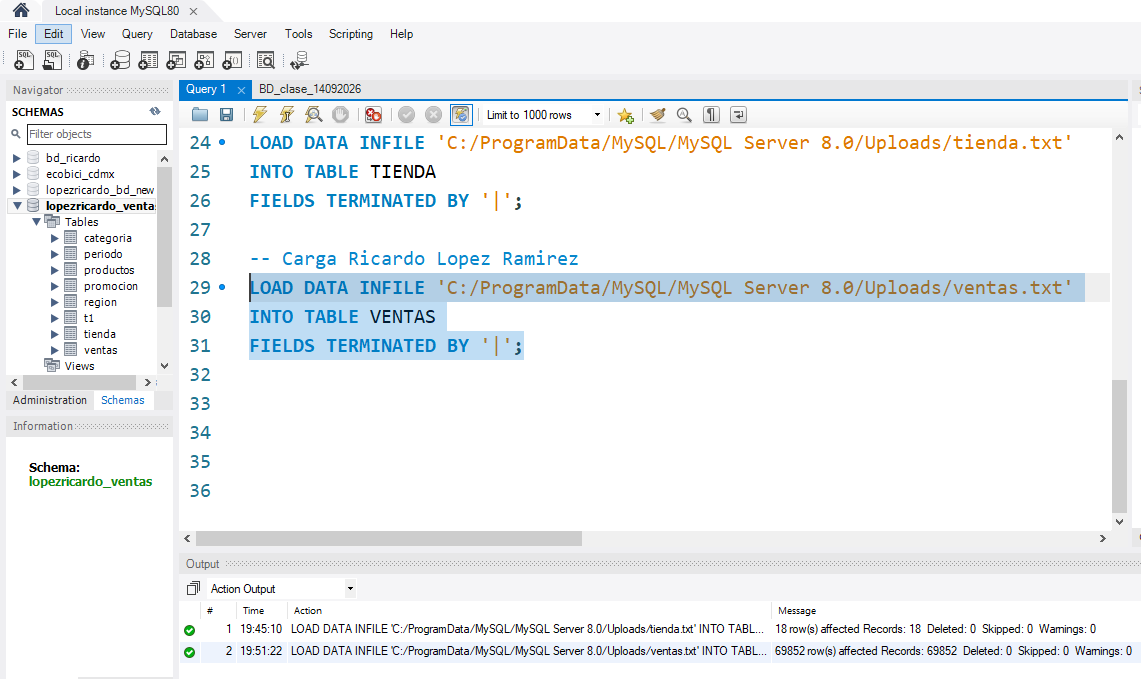
\includegraphics[
        width=0.8\textwidth
    ]{../Actividad_3/Imagen/ventas.png}
    \caption{Tabla ventas}
    \label{fig:tabla-ventas}
\end{figure}

\newpage

\section{Tablas con formato de fecha especial}

\subsection{Tabla \texttt{periodo}}

\vspace{2mm}

Las fechas se encuentran en formato \texttt{DD/MM/YYYY}.
Debido a que MySQL requiere un formato compatible con su
representación nativa de fechas, es necesario utilizar la
función \texttt{STR\_TO\_DATE()} para realizar la conversión
correspondiente.

\vspace{2mm}

donde \texttt{\%d} representa el día, \texttt{\%m} el mes y
\texttt{\%Y} el año.

\vspace{2mm}

\begin{figure}[H]
    \centering
    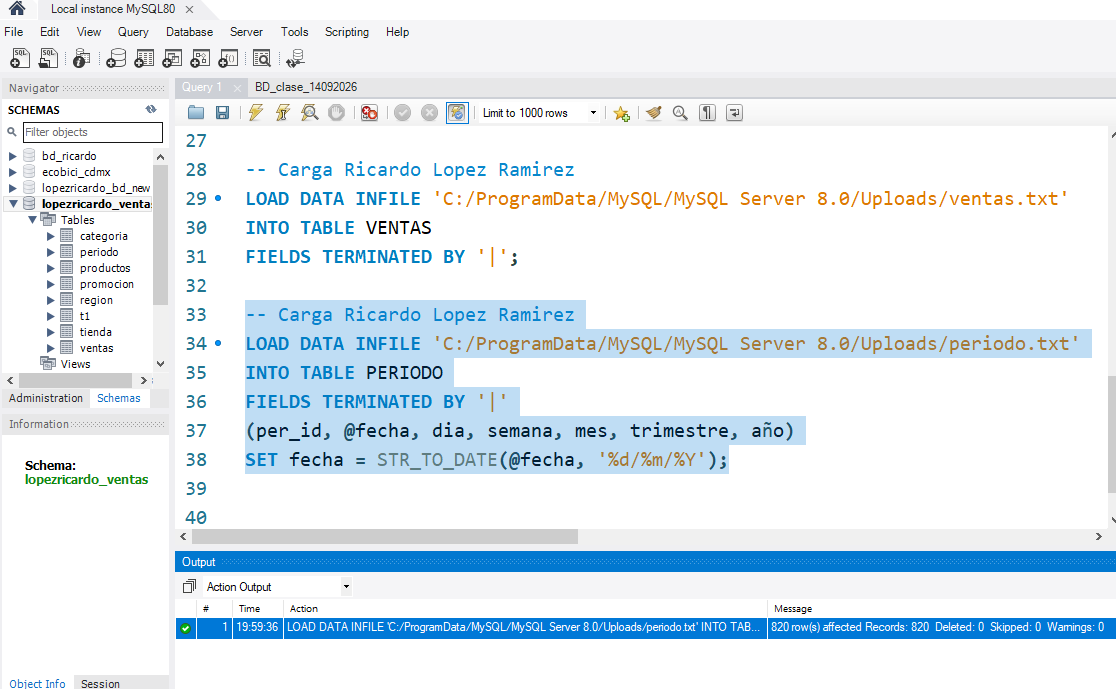
\includegraphics[
        width=0.8\textwidth
    ]{../Actividad_3/Imagen/periodo.png}
    \caption{Tabla periodo}
    \label{fig:tabla-periodo}
\end{figure}

\subsection{Tabla \texttt{promocion}}

\vspace{2mm}

\begin{figure}[H]
    \centering
    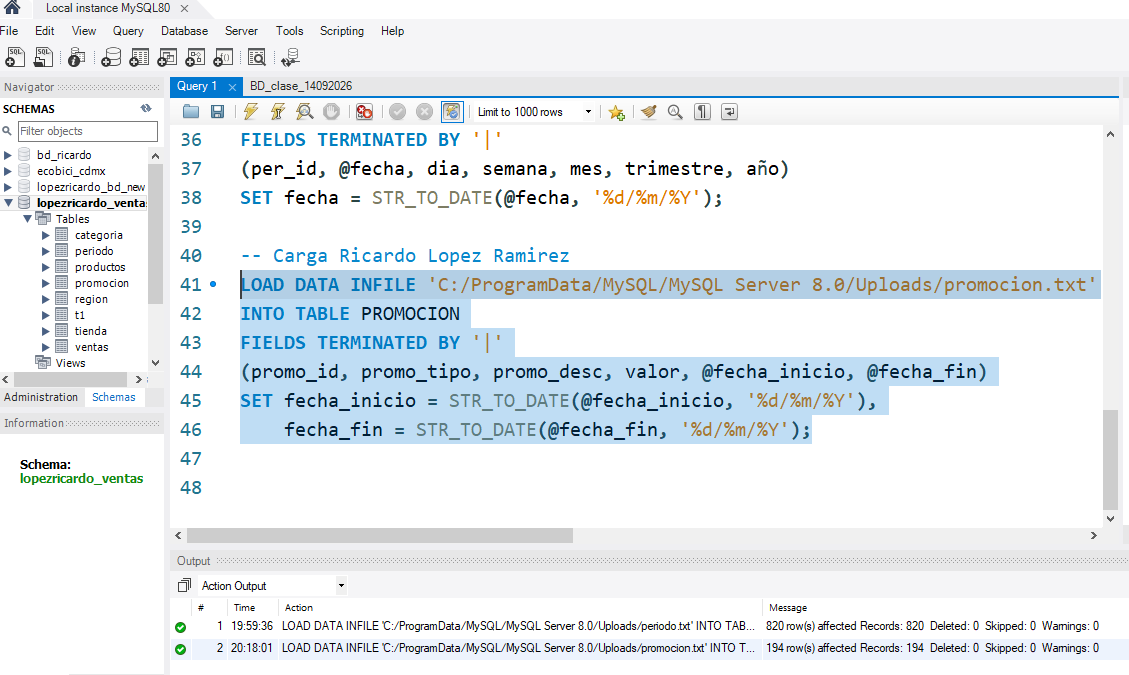
\includegraphics[
        width=0.8\textwidth
    ]{../Actividad_3/Imagen/promocion.png}
    \caption{Tabla promoción}
    \label{fig:tabla-promocion}
\end{figure}

\newpage
\section{Verificación y Conteo de Registros}

Usando el metodo UNION ALL: Junta los resultadoos de las
7 consultas y los consolida en una sola pestaña o tabla resumen.

\begin{figure}[H]
    \centering

    \begin{subfigure}{0.48\textwidth}
        \centering
        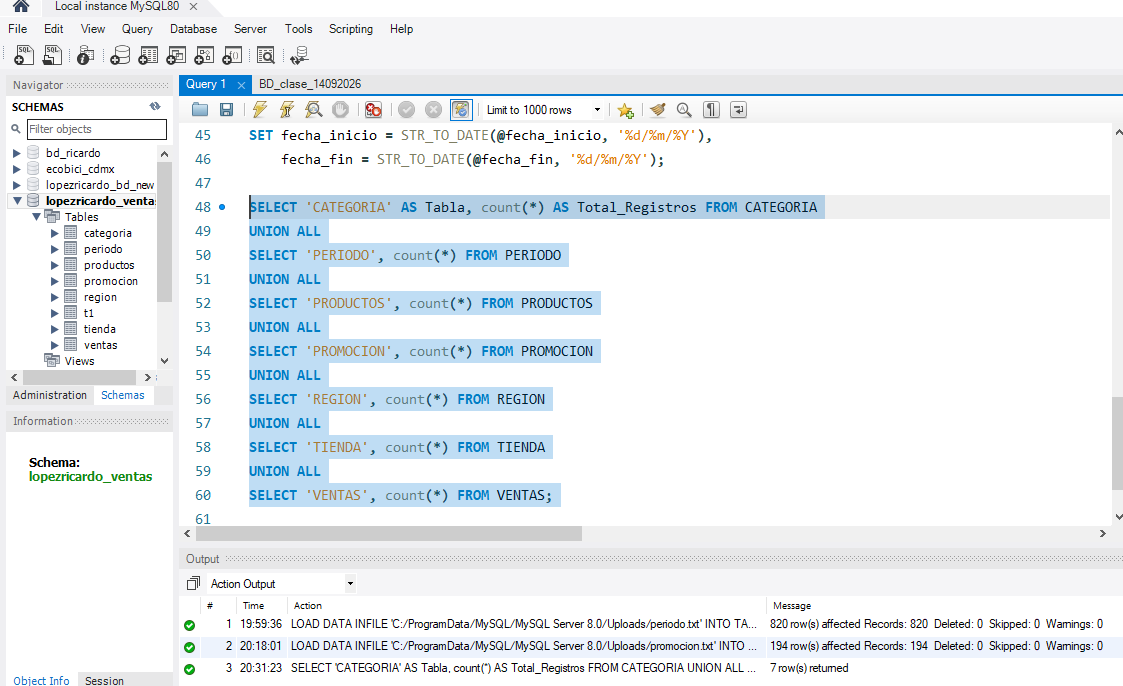
\includegraphics[width=\textwidth]{../Actividad_3/Imagen/VER1.png}
        \caption{Conteo de registros.}
        \label{fig:instalacion3}
    \end{subfigure}
    \hfill
    \begin{subfigure}{0.48\textwidth}
        \centering
        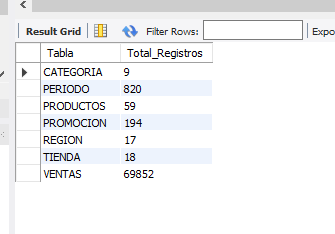
\includegraphics[width=\textwidth]{../Actividad_3/Imagen/VER2.png}
        \caption{Conteo de registros con UNION ALL.}
        \label{fig:instalacion4}
    \end{subfigure}

    \caption{Conteo de registros en las tablas.}
    \label{fig:Conteo-registros}
\end{figure}

\textbf{Verificación y Conteo de Registros Individuales:}


\begin{figure}[H]
    \centering

    \begin{subfigure}{0.48\textwidth}
        \centering
        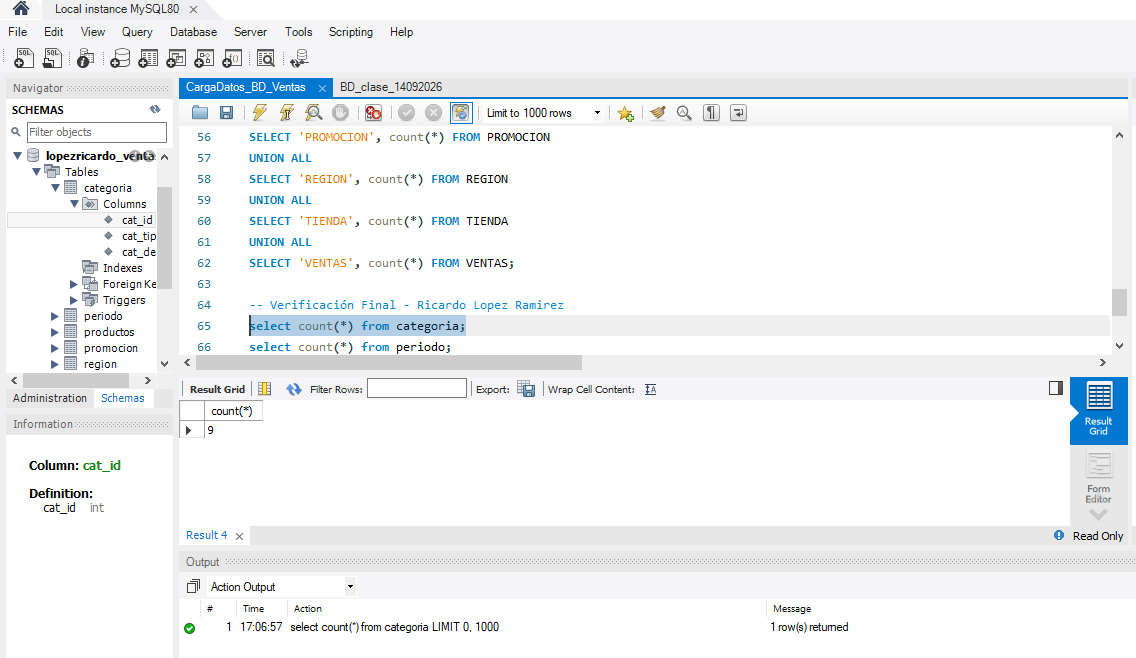
\includegraphics[width=\textwidth]{../Actividad_3/Imagen/T_categoria.PNG}
        \caption{17:06:57	select count(*) from categoria LIMIT 0, 1000	1 row(s) returned	0.031 sec / 0.000 sec
}
        \label{fig:instalacion7}
    \end{subfigure}
    \hfill
    \begin{subfigure}{0.48\textwidth}
        \centering
        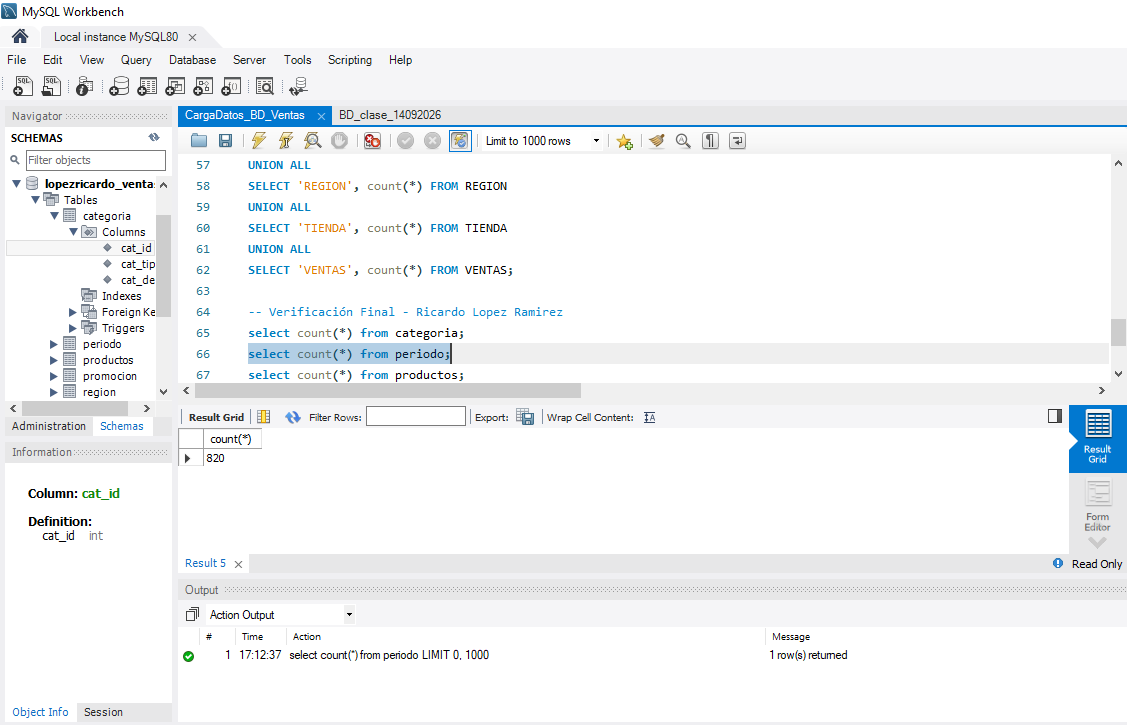
\includegraphics[width=\textwidth]{../Actividad_3/Imagen/T_periodo.PNG}
        \caption{17:12:37	select count(*) from periodo LIMIT 0, 1000	1 row(s) returned	0.031 sec / 0.000 sec
}
        \label{fig:instalacion8}
    \end{subfigure}

\end{figure}

\begin{figure}[H]
    \centering

    \begin{subfigure}{0.48\textwidth}
        \centering
        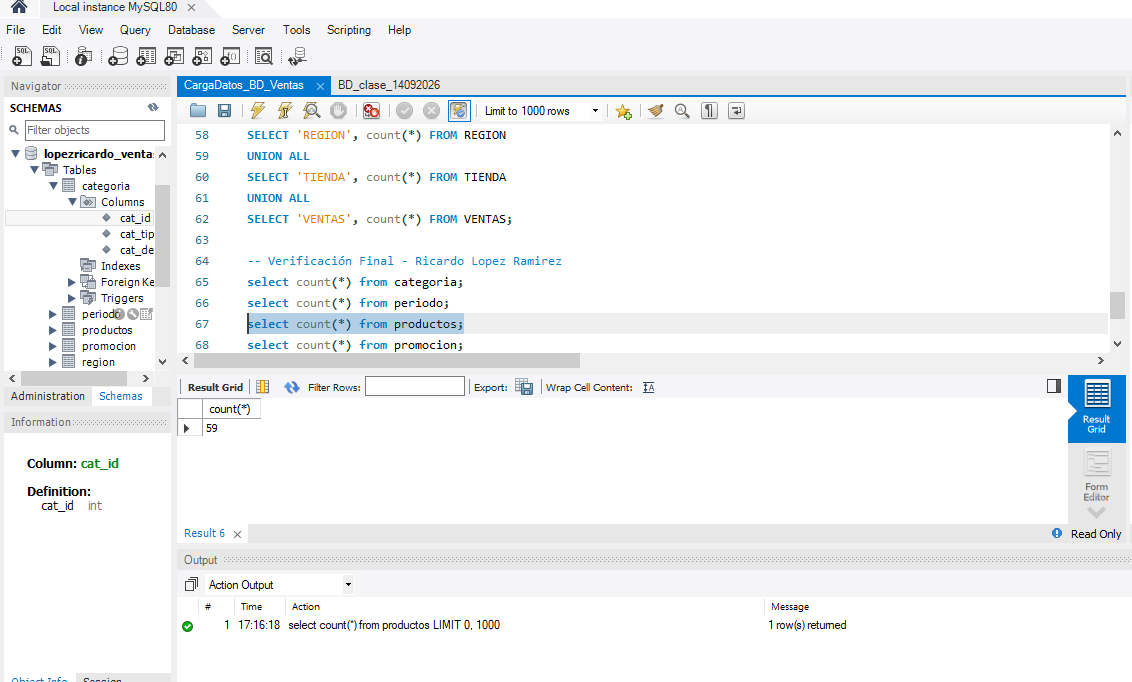
\includegraphics[width=\textwidth]{../Actividad_3/Imagen/T_productos.PNG}
        \caption{17:16:18	select count(*) from productos LIMIT 0, 1000	1 row(s) returned	0.031 sec / 0.000 sec
}
        \label{fig:instalacion9}
    \end{subfigure}
    \hfill
    \begin{subfigure}{0.48\textwidth}
        \centering
        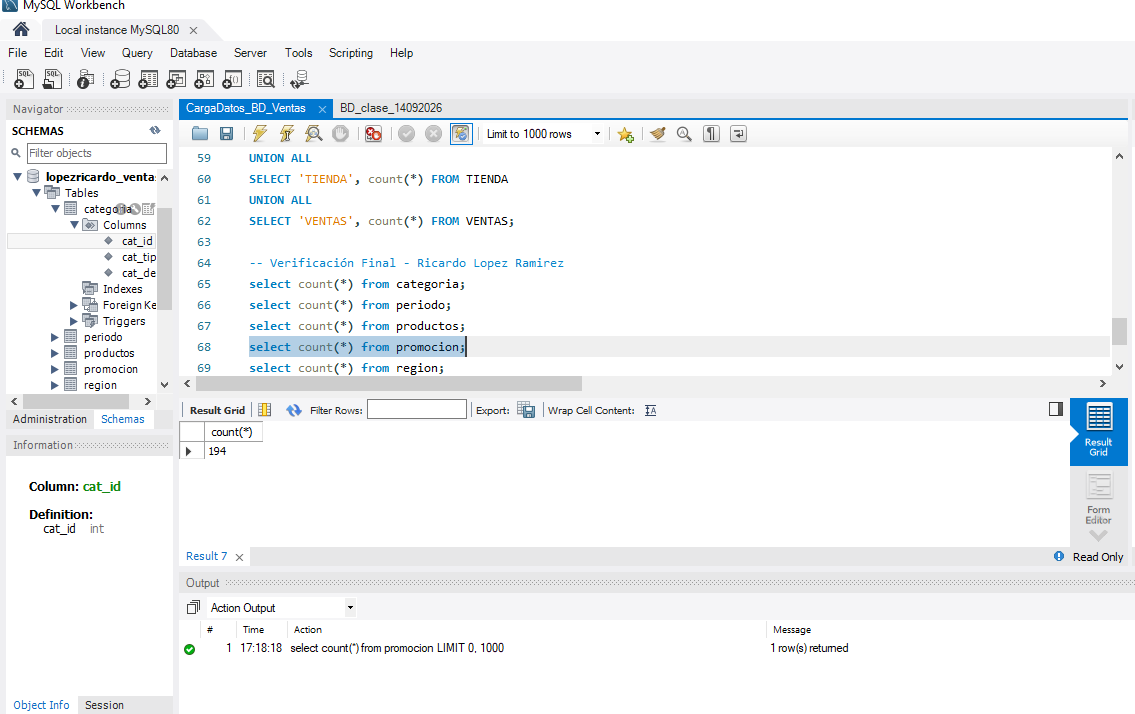
\includegraphics[width=\textwidth]{../Actividad_3/Imagen/T_promocion.PNG}
        \caption{17:18:18	select count(*) from promocion LIMIT 0, 1000	1 row(s) returned	0.016 sec / 0.000 sec
}
        \label{fig:instalacion10}
    \end{subfigure}

\end{figure}

\begin{figure}[H]
    \centering

    \begin{subfigure}{0.48\textwidth}
        \centering
        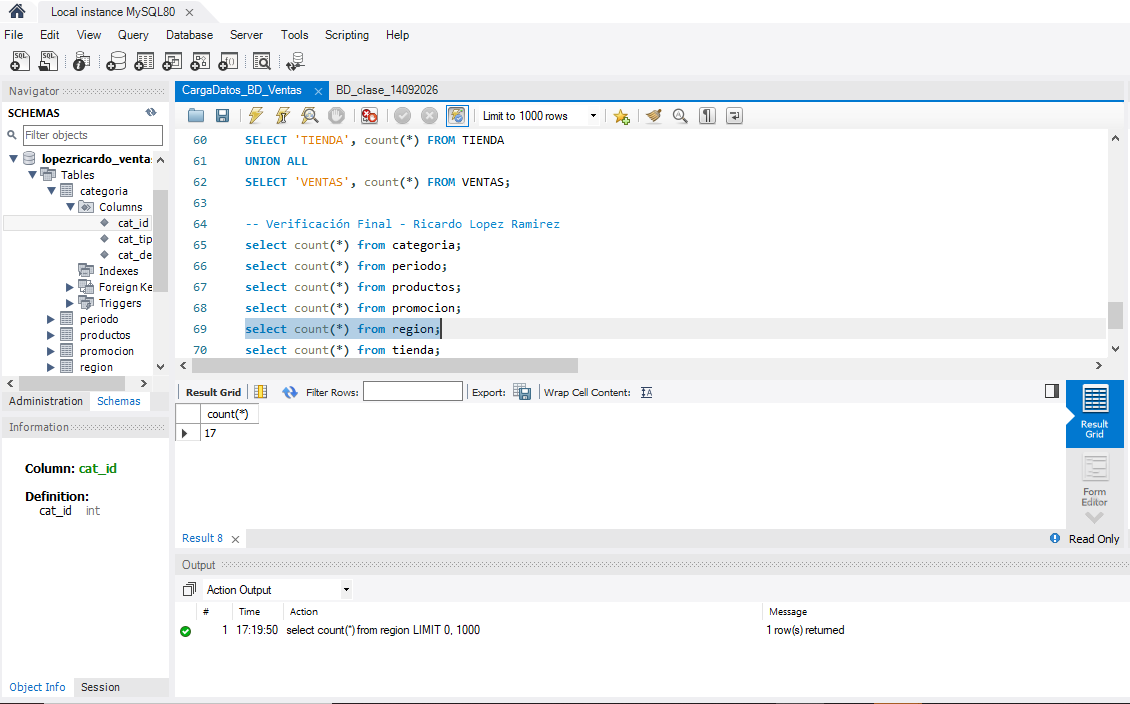
\includegraphics[width=\textwidth]{../Actividad_3/Imagen/T_region.PNG}
        \caption{17:19:50	select count(*) from region LIMIT 0, 1000	1 row(s) returned	0.031 sec / 0.000 sec
}
        \label{fig:instalacion11}
    \end{subfigure}
    \hfill
    \begin{subfigure}{0.48\textwidth}
        \centering
        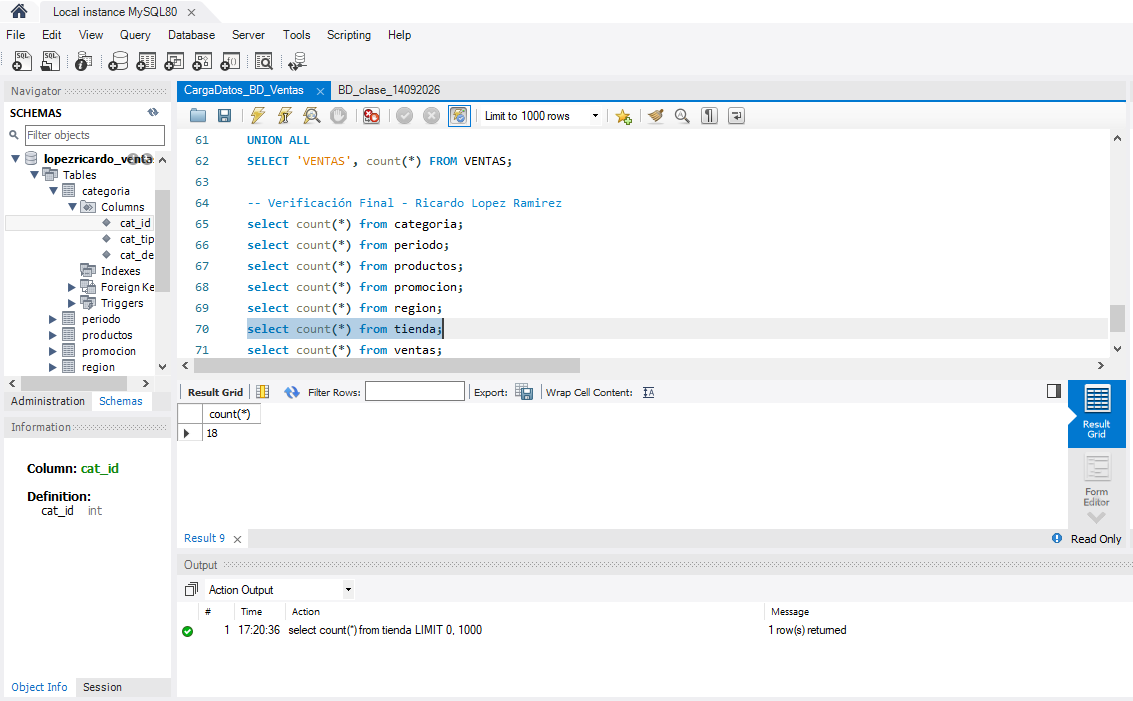
\includegraphics[width=\textwidth]{../Actividad_3/Imagen/T_tienda.PNG}
        \caption{17:20:36	select count(*) from tienda LIMIT 0, 1000	1 row(s) returned	0.125 sec / 0.000 sec
}
        \label{fig:instalacion12}
    \end{subfigure}

\end{figure}

\begin{figure}[H]
    \centering
    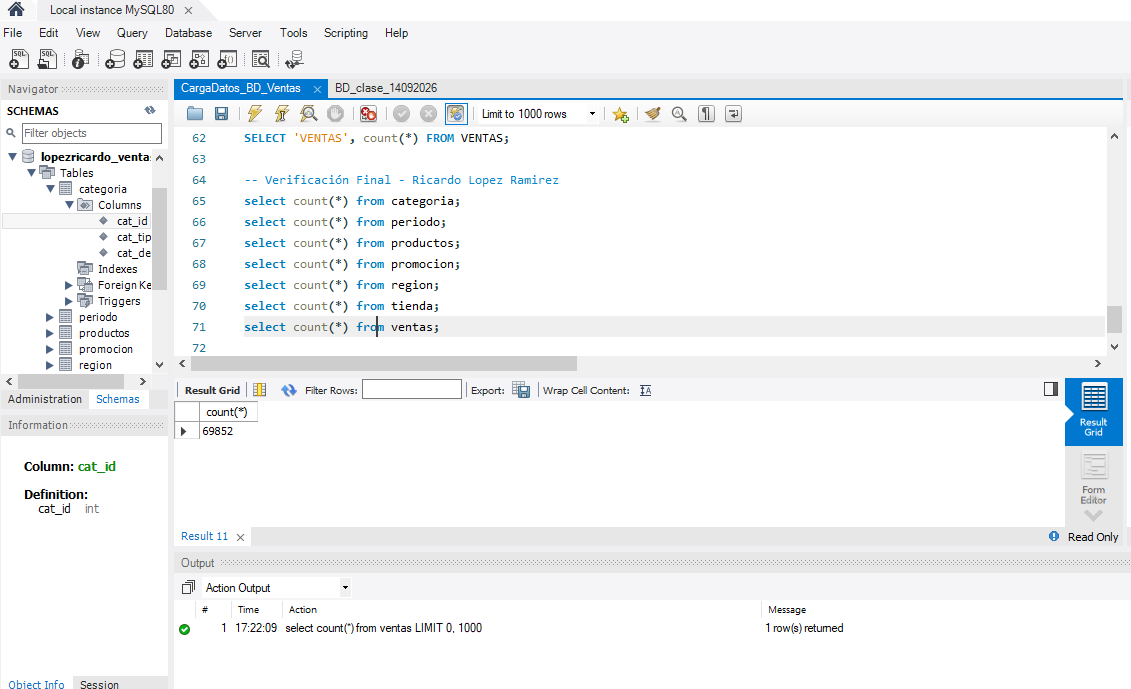
\includegraphics[
        width=0.8\textwidth
    ]{../Actividad_3/Imagen/T_ventas.PNG}
    \caption{17:22:09	select count(*) from ventas LIMIT 0, 1000	1 row(s) returned	0.047 sec / 0.000 sec
}
    \label{fig:tabla-ventas2}
\end{figure}


\newpage
\section{Referencias}

\renewcommand{\refname}{Referencias} % Cambia el título a "Referencias"
\begin{thebibliography}{99}

\bibitem{gemini2026}
Google. (2026). \textit{Gemini} (Large language model). https://gemini.google.com/

\bibitem{grippa2021}
Grippa, V. M., \& Kuzmichev, S. (2021). \textit{Learning MySQL: Get a handle on your data}. O'Reilly Media.

\bibitem{mysql80_bulk}
Oracle Corporation. (2024). \textit{MySQL 8.0 reference manual: 8.2.5.1 Optimizing INSERT statements}. https://dev.mysql.com/doc/refman/8.0/en/insert-optimization.html

\end{thebibliography}

\end{document}